\documentclass[12pt]{article}
\usepackage[utf8]{inputenc}
\usepackage{amsmath}
\usepackage{amssymb}
\usepackage{mathtools}
\usepackage{amsfonts}
\usepackage{lastpage}
\usepackage{tikz}
\usepackage{pdfpages}
\usepackage{gauss}
\usepackage{fancyvrb}
\usepackage{fancyhdr}
\usepackage{graphicx}
\pagestyle{fancy}
\fancyfoot[C]{\footnotesize Page \thepage\ of 3}
\DeclareGraphicsExtensions{.pdf,.png,.jpg}
\title{Elementær Talteori}
\author{Nikolaj Dybdahl Rathcke}
\chead{Nikolaj Dybdahl Rathcke (rfq695)}

\begin{document}
Vi kan opstille det karakteristiske polynomium
$$\lambda^3-3\lambda^2+4=0$$
Hvor af rødderne kan udregnes\\
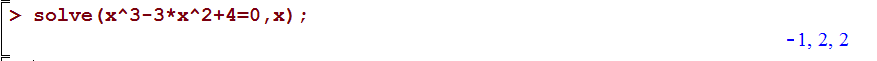
\includegraphics[width=\textwidth]{1}\\
og rodden $2$ har multiplicitet $2$, så $\lambda_1=-1$,$\lambda_2=2$ og $\lambda_3=2$.\\
Vi kan finde basis løsningerne til dette
\begin{align*}
x(-1)&=[\lambda_1^1,\lambda_1^2,\lambda_1^3,\lambda_1^4,...] \\
&=[-1,1,-1,1,...] \\
x(2)&=[\lambda_2^1,\lambda_2^2,\lambda_2^3,\lambda_2^4,...] \\
&=[2,4,8,16,...] \\
x'(2)&=[\frac{\partial}{\partial\lambda}\lambda_3^1,\frac{\partial}{\partial\lambda}\lambda_3^2,\frac{\partial}{\partial\lambda}\lambda_3^3,\frac{\partial}{\partial\lambda}\lambda_3^4,...] \\
&=[1\lambda_3^0,2\lambda_3^1,3\lambda_3^2,4\lambda_3^3,...] \\
&=[1,-2,3,-4,...]
\end{align*}
Altså har vi basis løsningerne
\begin{align*}
x_1&=[-1,1,-1,1,...] \\
x_2&=[2,4,8,16,...] \\
x_3&=[1,-2,3,-4,...]
\end{align*}


\end{document}
